\documentclass[border=5mm]{standalone}

\usepackage{pgfplots}

\begin{document}

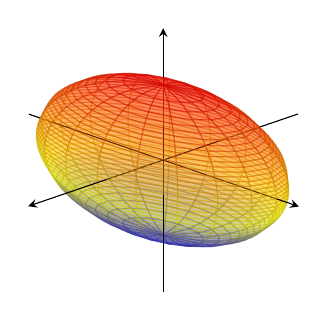
\begin{tikzpicture}
\begin{axis}
[view={135}{20},%colormap/blackwhite,
axis lines=center, axis on top, ticks=none,
set layers=default, axis equal,
%%xlabel={$x$}, ylabel={$y$}, zlabel={$z$},
xlabel style={anchor=south east},
ylabel style={anchor=south west},
zlabel style={anchor=south west},
enlargelimits,
tick align=inside,
domain=0:2.00,
samples=20, 
z buffer=sort,
]
\addplot3 [surf,opacity=0.4,domain=-1:0,
domain y=0:360] ({sin(y)*sqrt(1-x^2)},{2*cos(y)*sqrt(1-x^2)},{x});
\addplot3 [surf,opacity=0.4,domain=0:1,
domain y=0:360,on layer=axis foreground] ({sin(y)*sqrt(1-x^2)},{2*cos(y)*sqrt(1-x^2)},{x});
\end{axis}
\end{tikzpicture}

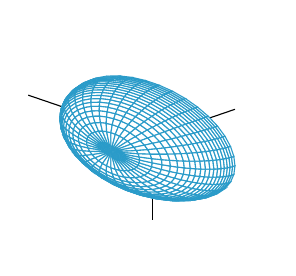
\begin{tikzpicture}[remember picture]
%\pgfsetlayers{pre main,main,axis foregound}
\begin{axis}
[view={135}{20},colormap={blue}{
            color=(cyan) color=(cyan)
        },axis lines=none,axis equal,set layers=standard,
enlargelimits,domain=0:2,samples=20, z buffer=sort,
]

\pgfonlayer{axis background}
\draw[-] (axis cs:0,0,-1.5)--(axis cs:0,0,-1);
\draw[-] (axis cs:0,-3,0)--(axis cs:0,-2,0);
\draw[-] (axis cs:-2,0,0)--(axis cs:-1,0,0);
\addplot3[draw=none] coordinates{(0,0,-2) (0,0,2)};
\addplot3[draw=none] coordinates{(0,-2.5,0) (0,2.8,0)};
\endpgfonlayer
\pgfonlayer{main}
\addplot3 [surf,draw=cyan,fill=white,domain=0:1,samples=20,
domain y=00:180] ({x},{-2*cos(y)*sqrt(1-x^2)},{-sin(y)*sqrt(1-x^2)});
\addplot3 [surf,draw=cyan,fill=white,domain=0:1,
domain y=0:180,on layer=axis foreground] ({x},{2*cos(y)*sqrt(1-x^2)},{sin(y)*sqrt(1-x^2)});
\coordinate(x1) at (axis cs:1,0,0);
\coordinate(x2) at (axis cs:1.5,0,0);
\coordinate(y1) at (axis cs:0,1.9,0);
\coordinate(y2) at (axis cs:0,2.5,0);
\coordinate(z1) at (axis cs:0,0,0.9);
\coordinate(z2) at (axis cs:0,0,1.5);
\endpgfonlayer
\end{axis}
\end{tikzpicture}

\begin{tikzpicture}[remember picture,overlay]
\draw[->] (x1)--(x2)node[left]{$x$};
\draw[->] (y1)--(y2)node[right]{$y$};
\draw[->] (z1)--(z2)node[right]{$z$};
\end{tikzpicture}

\end{document}
